\documentclass[10pt]{beamer}
\usepackage[utf8]{inputenc}
\usepackage{xeCJK}
\usepackage{graphicx}
\usepackage {mathtools}
\usepackage{utopia} %font utopia imported
\usetheme{CambridgeUS}
\usecolortheme{dolphin}
\usepackage{adjustbox}
\usepackage{subcaption}
% so that the captions are numerated
\setbeamertemplate{caption}[numbered]
\usepackage{xcolor}%[dvipsnames]
%\usepackage[hidelinks]{hyperref}
%\usetheme{Copenhagen}
%\newenvironment{vblock}[3]{%
%\setbeamercolor{block body}{#2}
%\setbeamercolor{body title}{#3}
%\begin{block}{#1}}{\end{block}}


% set colors
%\definecolor{myNewColorA}{RGB}{126,12,110}
%\definecolor{myNewColorB}{RGB}{165,85,154}
%\definecolor{myNewColorC}{RGB}{203,158,197}
\definecolor{myNewColorA}{RGB}{242,85,37}
\definecolor{myNewColorB}{RGB}{247,124,40}
\definecolor{myNewColorC}{RGB}{255,209,84}
\setbeamercolor*{palette primary}{bg=myNewColorC}
\setbeamercolor*{palette secondary}{bg=myNewColorB, fg = white}
\setbeamercolor*{palette tertiary}{bg=myNewColorA, fg = white}
\setbeamercolor*{titlelike}{fg=myNewColorA}
\setbeamercolor*{title}{bg=myNewColorA, fg = white}
\setbeamercolor*{item}{fg=myNewColorA}
\setbeamercolor*{caption name}{fg=myNewColorA}
%\setbeamercolor*{block body}{use=structure,fg=black,bg=myNewColorC}
\usefonttheme{professionalfonts}
\usepackage{natbib}
\usepackage{hyperref}
%------------------------------------------------------------
\titlegraphic{\includegraphics[height=2.2cm]{9019.jpg}}

\setbeamerfont{title}{size=\large}
\setbeamerfont{subtitle}{size=\small}
\setbeamerfont{author}{size=\small}
\setbeamerfont{date}{size=\small}
\setbeamerfont{institute}{size=\small}
\title{Estimating under-reporting of
COVID-19 cases in Indian states}
%\subtitle{MA4240 - Applied Statistics}
\author[MA4240 - Applied Statistics]{MA4240 - Applied Statistics}

\institute{IIT Hyderabad}
\date{April 26 2022}

%------------------------------------------------------------
%This block of commands puts the table of contents at the 
%beginning of each section and highlights the current section:
%\AtBeginSection[]
%{
%  \begin{frame}
%    \frametitle{Contents}
%    \tableofcontents[currentsection]
%  \end{frame}
%}
\AtBeginSection[]{
  \begin{frame}
  \vfill
  \centering
  \begin{beamercolorbox}[sep=8pt,center,shadow=true,rounded=true]{title}
    \usebeamerfont{title}\insertsectionhead\par%
  \end{beamercolorbox}
  \vfill
  \end{frame}
}
%------------------------------------------------------------

\begin{document}

%The next statement creates the title page.
\frame{\titlepage}
\begin{frame}{Team Members}
    \begin{itemize}
        \item Adepu Adarsh Sai - AI20BTECH11001
        \item Ananthoju Pranav Sai - AI20BTECH11004
        \item Murarisetty Adhvik - AI20BTECH11015
        \item Perambuduri Srikaran - AI20BTECH11018
        \item Arun Siddardha - AI20BTECH11019
        \item Yashas Tadikamalla - AI20BTECH11027
    \end{itemize}
\end{frame}
\begin{frame}
\frametitle{Contents}
\tableofcontents
\end{frame}
%------------------------------------------------------------
\section{Introduction}
\begin{frame}{Introduction}
\begin{itemize}
    \item It is observed that there has been a significant under-reporting in COVID-19 cases in India. Some of the possible reasons for this are:
\begin{itemize}
    \item Low testing coverage
    \item Asymptomatic cases
\end{itemize}
    \item We try to obtain both, an average as well as a time varying estimate for the fraction of COVID-19 cases reported in each state of India.
    \item The former is calculated using a delay adjusted case fatality ratio (CFR) approach for different states, while the latter is obtained by modelling the problem as a time-varying Poisson process.
\end{itemize}
\end{frame} 
\section{Definitions}
\subsection{Log-Normal Distribution}
\begin{frame}{Log-Normal Distribution}
    \begin{itemize}
        \item A log-normal distribution is a continuous probability distribution of a random variable whose logarithm is normally distributed. 
    \end{itemize}
    \begin{block}{}
    The PDF of $X \sim {\displaystyle \operatorname {Lognormal} (\mu ,\,\sigma ^{2})}$ is given by 
    \begin{align}
        {f_X(x) =  {\frac {1}{x\sigma {\sqrt {2\pi }}}}\ \exp \left(-{\frac {\left(\ln \left(x\right)-\mu \right)^{2}}{2\sigma ^{2}}}\right)}
    \end{align}
    \end{block}
    \begin{itemize}
        \item ${\mathbb{E}[X]} = {\displaystyle \exp \left(\mu +{\frac {\sigma ^{2}}{2}}\right)}$, \hspace{4mm} $Var[X] = {\displaystyle [e^{(\sigma ^{2})}-1]e^{(2\mu +\sigma ^{2})}}$
        \item The length of chess games tends to follow a log-normal distribution.
    \end{itemize}
\end{frame}
\subsection{Poisson Distribution}
\begin{frame}{Poisson distribution}
    \begin{block}{}
    A discrete random variable $X$ is said to be a Poisson random variable with parameter $\lambda$, shown as $X \sim Poisson(\lambda)$, if its range is $R_X={0,1,2,3,...}$, and its PMF is given by
    \begin{align}
        P_X(k)=\begin{cases}
        \frac{e^{-\lambda}\lambda^{k}}{k!} & \text{for } k \in R_X \\
        0 & \text{otherwise}
        \end{cases}
    \end{align}
    \end{block}
    \begin{itemize}
        \item If $X\sim Poisson(\lambda)$, then $E[X]=\lambda$, and $Var(X)=\lambda$.
    \end{itemize}
\end{frame}
\subsection{Time-varying Poisson Process}
\begin{frame}{Time-varying Poisson process}
    \begin{itemize}
        \item Poisson process is most commonly used in cases when we're counting the number of times certain events appear to occur at a specific rate, but, are truly random.
        % \item Let $\lambda>0$ be fixed. The counting process $N(t)$, $t\in [0,\infty)$ is called a Poisson process with rates $\lambda$ if all the following conditions hold:
        % \begin{itemize}
        %     \item $N(0)=0$
        %     \item $N(t)$ has independent increments
        %     \item The number of arrivals in any interval of length $\tau>0$ has Poisson($λ\lambda \tau$) distribution.
        % \end{itemize}
        \item A time varying Poisson process is a Poisson process whose event rate $\lambda$ varies with time. 
        \item The probability of an event occuring k times in a time interval with event rate $\lambda_t$ is \begin{align}
            P_{X}(k)=\frac{e^{-\lambda_t}\lambda_t^{k}}{k!}
        \end{align}
    \end{itemize}
\end{frame}
\subsection{Poisson Regression}
\begin{frame}{Poisson Regression}
    \begin{itemize}
        \item Poisson regression is a generalized linear model form of regression analysis used to model count data and contingency tables.
        \item Poisson regression assumes the response variable $Y$ has a Poisson distribution, and assumes the logarithm of its expected value can be modeled by a linear combination of unknown parameters. 
        \item If  $\mathbf {\underline{x}_t} \in \mathbb {R} ^{n}$ is a vector of explanatory variables, then we can model $\lambda_t$ as
        \begin{align}
            \log (\lambda_t) = \alpha + \underline{\beta}^{\top}\underline{x}_{t}
        \end{align}
        where $\alpha \in \mathbb{R}$, $\beta \in \mathbb{R}^{n}$
        \item Hence,
        \begin{align}
            PMF(Y_t/\underline{x}_t)=\frac{e^{-\lambda_t}\lambda_t^{Y_t}}{Y_t!}
        \end{align}
    \end{itemize}
\end{frame}
\begin{frame}{Poisson Regression}
    \begin{itemize}
    \item The log-likelihood of the data is given by 
    \begin{align}
        ln (L(\underline{\beta}))=\displaystyle\sum_{t}(Y_t\underline{x}_t\underline{\beta}-e^{x_t\underline{\beta}}-lnY_t!)
    \end{align}
        \item We use Maximum Likelihood Estimation to find the coefficients $\beta$ of the regression model
        \begin{align}
            \displaystyle\sum_{t}(Y_t-e^{\underline{x}_t\underline{\beta}})\underline{x}_t=0
        \end{align}
        \item Solving this, will give the coefficients $\underline{\beta}$.
    \end{itemize}
\end{frame}
\section{Data and Key Assumptions}
\begin{frame}{Data and Key Assumptions}
  \begin{itemize}
      \item The data is taken from \href{https://www.covid19india.org/}{\color{blue}{covid19india.org}}. It consists of the number of cases reported and the number of deaths on each day for every state in India.
      \item Some of the assumptions we assumed to perform the analysis are:
\begin{itemize}
    \item Deaths due to COVID-19 are reported accurately i.e., no under-reporting of deaths.
    \item For fatal cases, the distribution of delay from confirmation to death is the same as the distribution of hospitalisation to death. We assume it is a log-normal distribution with mean of 13 days and standard deviation of 12.7 days. %\cite{8}
\end{itemize}
\item We will use the baseline CFR value as 0.1\%.
  \end{itemize}  
\end{frame}
\section{Average estimate of fraction of cases reported}
\begin{frame}{Average estimate of fraction of cases reported}
    \begin{itemize}
        \item Naive CFR can be calculated as
        \begin{align}
            nCFR = \frac{\text{deaths-to-date}}{\text{cases-to-date}}
        \end{align}
        This is clearly inaccurate as the additional deaths that may arise from the cases observed to date will not be counted.
        \item Hence, we can use the distribution of delay from hospitalisation to calculate the delay-adjusted CFR as ratio of deaths to the expected number of eventually fatal cases.
        \begin{align}
    cCFR = \frac{\sum_{t=0}^{T}d_t}{\sum_{t=0}^{T}\sum_{s<t}p_{t-s}c_s}
\end{align}
Here, $d_t$ and $c_t$ are the number of new deaths and the number of new cases reported on day $t$ from a certain region respectively. $p_s$ is the probability that an eventually fatal case will lead to death on the $s^{\text{th}}$ day from the day of reporting. $T$ is the last day for which the data is available.
    \end{itemize}
\end{frame}

\begin{frame}{Average estimate of fraction of cases reported}
    \begin{itemize}
        \item In regions where the cases have been under reported, the adjusted CFR will be higher than the true CFR. So, calculating the ratio of the true CFR to the adjusted CFR will give an estimate of the fraction of cases reported.
\begin{align}
    f_{avg} = \frac{CFR}{cCFR}
\end{align}
\item The expected total number of deaths to occur among the reported cases on day $t$ can be written as,
\begin{align}
    e_t = \sum_{s<t}p_{t-s}c_{s}.CFR
\end{align}
Here, $CFR$ is the true CFR which we assumed at the start of the analysis.
    \end{itemize}
\end{frame}

\begin{frame}{Average estimate of fraction of cases reported}
    \begin{itemize}
\item The ratio of $\sum_{t=0}^{T}e_t$ to the number of deaths reported by day $T$ gives the average fraction of true cases that have been reported in a region over the complete time period.
\begin{align}
    f_{avg} = \frac{\sum_{t}e_t}{\sum_{t}d_t} 
\end{align}
    \end{itemize}
\end{frame}
\section{Time varying estimate of fraction of cases reported}
\begin{frame}{Time varying estimate of true fraction of cases}
        \begin{itemize}
            \item We can further improve the estimate to obtain a time varying estimate of the fraction of cases reported.
            \item We model the number of daily deaths as a time-varying Poisson process. The number of deaths on day $t$ is a random Poisson variable with mean,
\begin{align}
    \lambda_t = \frac{e_t}{f_t} \label{eq:1}
\end{align}
Here, $f_t$ is the fraction of cases reported on day $t$
        \end{itemize}
\end{frame}
\begin{frame}{Time varying estimate of fraction of cases reported}
    \begin{itemize}
        \item We estimate $\lambda_t$ by performing Poisson regression on daily death cases. Subsequently we can find $f_t$ using \eqref{eq:1}.
        \begin{align}
            \log (\lambda_t) = b_0 + b_1(t) + b_2(c_t)
        \end{align}
        where $c_t$ is the number of cases reported on day $t$.
        
    \item Estimate of daily fraction of reported cases is given by
    \begin{align}
        f_t = \frac{e_t}{\lambda_t}
    \end{align}
    \end{itemize}
\end{frame}
\section{Confidence Interval bounds}
\begin{frame}{Confidence Interval bounds}
    \begin{itemize}
        \item Let $X_1,X_2,..,X_n$ be a random sample from a normal distribution with mean $\mu$ and variance $\sigma^2$.Then the 95\% CI for the mean $\mu$ is given by
        \begin{align}
            \overline{x} \pm 1.96\sqrt{\frac{\sigma^2}{n}}
        \end{align}
        \item Using CLT, we can claim that the 95\% CI for $\lambda_t$ will be
        \begin{align}
    {\lambda_t} \pm 1.96\sqrt{\frac{{\lambda_t}}{n}}
\end{align}
where $n$ is the the total number of days.
\begin{align}
    \text{95\% CI for $\lambda_t$} &= \left(\lambda_t-1.96\sqrt{\frac{\lambda_t}{n}},\lambda_t+1.96\sqrt{\frac{\lambda_t}{n}} \right)
\end{align}
    \end{itemize}
\end{frame}
% \begin{frame}{95\% CI interval for $f_t$}
%     \begin{align}
%         \text{95\% CI for $\lambda_t$} &= \left(\lambda_t-1.96\sqrt{\frac{\lambda_t}{n}},\lambda_t+1.96\sqrt{\frac{\lambda_t}{n}} \right)\\
%         \text{Since } f_t=\frac{e_t}{\lambda_t}&\\
%         \text{95\% CI for $f_t$} &= 
%         \left(\frac{e_t}{\lambda_t+1.96\sqrt{\frac{\lambda_t}{n}}} , \frac{e_t}{\lambda_t-1.96\sqrt{\frac{\lambda_t}{n}}}\right) \label{eq:17}
%     \end{align}
%     Using \eqref{eq:17} we can find 95\% CI intervals for each estimate of $f_t$.
% \end{frame}
\section{Results and Observations}
\begin{frame}{Results}
    \begin{itemize}
        \item The codes can be found  \href{https://github.com/Ananthoju-Pranav-Sai/MA4240_Project}{\color{blue}here}.
        \item Average and time-varying estimate of fraction of cases
        \begin{center}
\begin{table}[!htp]
\begin{adjustbox}{width=0.85\columnwidth}
\scalebox{1.1}{

\begin{tabular}{|l|l|l|l|l|l|}
\hline
\textbf{\begin{tabular}[c]{@{}l@{}}State\\ /country\end{tabular}} & \textbf{Deaths} & \textbf{Cases} & \textbf{\begin{tabular}[c]{@{}l@{}}nCFR\\  (\%)\end{tabular}} & \textbf{\begin{tabular}[c]{@{}l@{}}cCFR\\  (\%)\end{tabular}} & \textbf{\begin{tabular}[c]{@{}l@{}}Percentage \\ Reported (\%)\end{tabular}} \\ \hline
India                                                             & 107459          & 6976461        & 1.54                                                          & 1.78                                                          & 5.60                                                                         \\ \hline
Telangana                                                         & 1208            & 208025         & 0.58                                                          & 0.65                                                          & 15.32                                                                        \\ \hline
Maharashtra                                                       & 39731           & 1506018        & 2.64                                                          & 3.01                                                          & 3.32                                                                         \\ \hline
Bihar                                                             & 934             & 193826         & 0.48                                                          & 0.52                                                          & 19.05                                                                        \\ \hline
Delhi                                                             & 5692            & 303693         & 1.87                                                          & 2.04                                                          & 4.91                                                                         \\ \hline
Kerala                                                            & 3773            & 122459         & 3.08                                                          & 3.66                                                          & 2.73                                                                         \\ \hline
\end{tabular}
}
\end{adjustbox}
\end{table}
\end{center}
\item There has been a major under-reporting, as indicated by the last column.
    \end{itemize}
\end{frame}
\begin{frame}{The fraction of cases reported in various regions as a function of time, assuming
a baseline CFR of 0.1\%}
 \begin{figure}
\centering
    \begin{subfigure}[tl]{0.3\textwidth}
        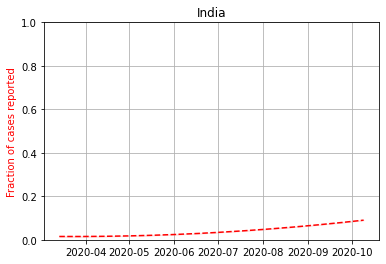
\includegraphics[width=\textwidth]{India.png}
        %\caption{Plot of fraction of cases reported vs }
        \label{fig:nature1}
    \end{subfigure}
    \begin{subfigure}[tc]{0.3\textwidth}
        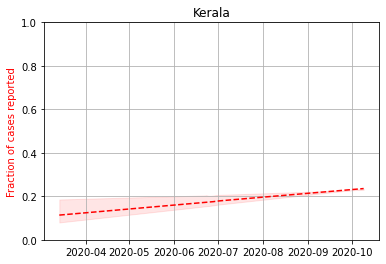
\includegraphics[width=\textwidth]{Kerala.png}
        %\caption{Image of the nature V2.}
        \label{fig:nature2}
    \end{subfigure}
    \begin{subfigure}[tr]{0.3\textwidth}
        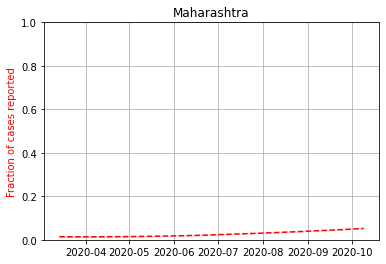
\includegraphics[width=\textwidth]{Maharashtra.png}
        %\caption{Image of the nature V2.}
        \label{fig:nature2}
    \end{subfigure}
    \begin{subfigure}[bl]{0.3\textwidth}
        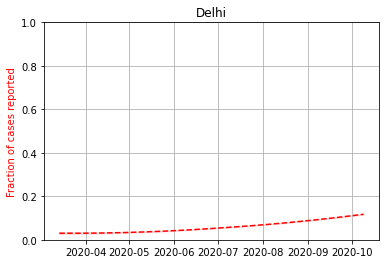
\includegraphics[width=\textwidth]{Delhi.png}
        %\caption{Image of the nature V2.}
        \label{fig:nature2}
    \end{subfigure}
    \begin{subfigure}[bc]{0.3\textwidth}
        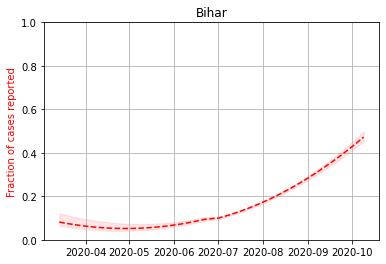
\includegraphics[width=\textwidth]{Bihar.png}
        %\caption{Image of the nature V2.}
        \label{fig:nature2}
    \end{subfigure}
    \begin{subfigure}[br]{0.3\textwidth}
        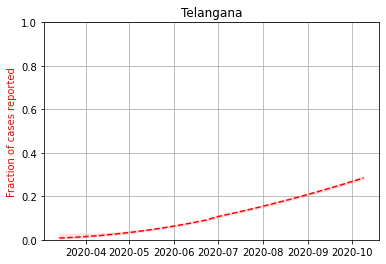
\includegraphics[width=\textwidth]{Telangana.png}
        %\caption{Image of the nature V2.}
        \label{fig:nature2}
    \end{subfigure}
%\caption{The fraction of cases reported in various regions as a function of time, assuming
%a baseline CFR of 0.1\%}
\label{fig:images}
\end{figure}
\end{frame}
\begin{frame}{Observations}
    \begin{itemize}
        \item It is observed that there has been a significant under-reporting during $2^{nd}$ wave of COVID-19 across India. The shaded region represents the interval of second wave. Here are a few plots
    \end{itemize}
     \begin{figure}
\centering
    \begin{subfigure}[tl]{0.4\textwidth}
        \includegraphics[width=\textwidth]{India2.png}
        %\caption{Plot of fraction of cases reported vs }
        \label{fig:nature1}
    \end{subfigure}
    % \begin{subfigure}[tr]{0.4\textwidth}
    %     \includegraphics[width=\textwidth]{Kerala2.png}
    %     %\caption{Image of the nature V2.}
    %     \label{fig:nature2}
    % \end{subfigure}
    \begin{subfigure}[bl]{0.4\textwidth}
        \includegraphics[width=\textwidth]{Maharashtra2.png}
        %\caption{Image of the nature V2.}
        \label{fig:nature2}
    \end{subfigure}
    % \begin{subfigure}[bl]{0.3\textwidth}
    %     \includegraphics[width=\textwidth]{delhi2.png}
    %     %\caption{Image of the nature V2.}
    %     \label{fig:nature2}
    % \end{subfigure}
    % \begin{subfigure}[bc]{0.3\textwidth}
    %     \includegraphics[width=\textwidth]{AP2.png}
    %     %\caption{Image of the nature V2.}
    %     \label{fig:nature2}
    % \end{subfigure}
    \begin{subfigure}[br]{0.4\textwidth}
        \includegraphics[width=\textwidth]{Telangana2.png}
        %\caption{Image of the nature V2.}
        \label{fig:nature2}
    \end{subfigure}
\label{fig:images}
\end{figure}
\end{frame}
\begin{frame}{Strengths and limitations of the study}
    Strengths:
    \begin{itemize}
     \item In states where extensive testing is infeasible, this study provides a method to quantify the true extent of spread of COVID-19.
    \item It provides important information, of trends of under-reporting in different states, which could be used for policy making.
    \end{itemize}
    Limitations:
    \begin{itemize}
    \item The accuracy of these results depends greatly on the quality
of the data and the assumptions being made.
    \end{itemize}
\end{frame}
\begin{frame}{References}
\begin{enumerate}
\item  Jayakrishnan Unnikrishnan, Sujith Mangalathu and  Raman V Kutty, "Estimating under-reporting of 
COVID-19 cases in Indian states: an 
approach using a delay-adjusted case 
fatality ratio", 2020.
\item Ioannidis J., "The infection fatality rate of COVID-19 inferred from 
seroprevalence data", 2020.
\item Linton NM, Kobayashi T, Yang Y, et al. "Incubation period and other epidemiological characteristics of 2019 novel coronavirus infections with right truncation: a statistical analysis of publicly available case data", 2020.
\end{enumerate}
\end{frame}
\begin{frame}
   \centering
    \textcolor{orange}{\Huge{\textbf{THANK YOU!}}}
\end{frame}

\end{document}



